\clearpage
\title{Problem 4.5}
\author{}
\date{}
\maketitle

\section*{Problem Description}

\section*{Process}
\subsection*{Code:}

\begin{multicols}{2}{|}
    \begin{minted}[linenos,breaklines,breakanywhere]{nasm}
DATA SEGMENT
    CR EQU 0DH
    LF EQU 0AH
    STARS DB CR, LF, "**********$"
    COUNTER DW 10
DATA ENDS  

CODE SEGMENT
    ASSUME CS:CODE, DS DATA

START:
    MOV AX, DATA
    MOV DS, AX
    MOV CX, COUNTER
    
LOOP_START:
    LEA DX, STARS
    MOV AH, 9
    INT 21H
    
    DEC CX
    CMP CX, 0 
    
    JE LOOP_END
    JMP LOOP_START 
    
LOOP_END:
    MOV AH, 4CH
    INT 21H 
    
CODE ENDS
END START
    \end{minted}
\end{multicols}

\subsection*{Output}
\begin{center}
    \centering
    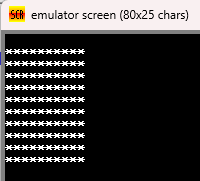
\includegraphics[width = .4\textwidth]{5.png}
    \captionof{figure}{Printing a pattern using Loop}
\end{center}
